\chapter{Development Tools \& Continuous Integration}
\label{ch:testing}

The following chapter will introduce a few tools included in the framework to ease development and help to maintain a high code quality. This comprises tools for the developer to be used while coding, as well as a continuous integration (CI) and automated test cases of various framework and module functionalities.

The chapter is structured as follows.
Section~\ref{sec:targets} describes the available \command{make} targets for code quality and formatting checks, Section~\ref{sec:ci} briefly introduces the CI, and Section~\ref{sec:tests} provides an overview of the currently implemented framework, module, and performance test scenarios.

\section{Additional Targets}
\label{sec:targets}

A set of testing targets in addition to the standard compilation targets are automatically created by CMake to enable additional code quality checks and testing.
Some of these targets are used by the project's CI, others are intended for manual checks.
Currently, the following targets are provided:

\begin{description}
  \item[\command{make format}] invokes the \command{clang-format} tool to apply the project's coding style convention to all files of the code base. The format is defined in the \file{.clang-format} file in the root directory of the repository and mostly follows the suggestions defined by the standard LLVM style with minor modifications. Most notably are the consistent usage of four whitespace characters as indentation and the column limit of 125 characters.
  \item[\command{make check-format}] also invokes the \command{clang-format} tool but does not apply the required changes to the code. Instead, it returns an exit code 0 (pass) if no changes are necessary and exit code 1 (fail) if changes are to be applied. This is used by the CI.
  \item[\command{make lint}] invokes the \command{clang-tidy} tool to provide additional linting of the source code. The tool tries to detect possible errors (and thus potential bugs), dangerous constructs (such as uninitialized variables) as well as stylistic errors. In addition, it ensures proper usage of modern C++ standards. The configuration used for the \command{clang-tidy} command can be found in the \file{.clang-tidy} file in the root directory of the repository.
  \item[\command{make check-lint}] also invokes the \command{clang-tidy} tool but does not report the issues found while parsing the code. Instead, it returns an exit code 0 (pass) if no errors have been produced and exit code 1 (fail) if issues are present. This is used by the CI.
  \item[\command{make cppcheck}] runs the \command{cppcheck} command for additional static code analysis. The output is stored in the file \file{cppcheck_results.xml} in XML2.0 format. It should be noted that some of the issues reported by the tool are to be considered false positives.
  \item[\command{make cppcheck-html}] compiles a HTML report from the defects list gathered by \command{make cppcheck}. This target is only available if the \command{cppcheck-htmlreport} executable is found in the \dir{PATH}.
  \item[\command{make package}] creates a binary release tarball as described in Section~\ref{sec:packaging}.
\end{description}

\section{Packaging}
\label{sec:packaging}
\apsq comes with a basic configuration to generate tarballs from the compiled binaries using the CPack command. In order to generate a working tarball from the current \apsq build, the \parameter{RPATH} of the executable should not be set, otherwise the \command{allpix} binary will not be able to locate the dynamic libraries. If not set, the global \parameter{LD_LIBRARY_PATH} is used to search for the required libraries:

\begin{verbatim}
$ mkdir build
$ cd build
$ cmake -DCMAKE_SKIP_RPATH=ON ..
$ make package
\end{verbatim}

Since the CMake installation path defaults to the project's source directory, certain files are excluded from the default installation target created by CMake.
This includes the detector models in the \dir{models/} directory as well as the additional tools provided in \dir{tools/root_analysis_macros/} folder. In order to include them in a release tarball produced by CPack, the installation path should be set to a location different from the project source folder, for example:

\begin{verbatim}
$ cmake -DCMAKE_INSTALL_PREFIX=/tmp ..
\end{verbatim}

The content of the produced tarball can be extracted to any location of the file system, but requires the ROOT6 and Geant4 libraries as well as possibly additional libraries linked by individual at runtime.

For this purpose, a \file{setup.sh} shell script is automatically generated and added to the tarball.
By default, it contains the ROOT6 path used for the compilation of the binaries.
Additional dependencies, either library paths or shell scripts to be sourced, can be added via CMake for individual modules using the CMake functions described below.
The paths stored correspond to the dependencies used at compile time, it might be necessary to change them manually when deploying on a different computer.

\paragraph{\texttt{\textbf{ADD\_RUNTIME\_DEP(name)}}}

This CMake command can be used to add a shell script to be sourced to the setup file.
The mandatory argument \parameter{name} can either be an absolute path to the corresponding file, or only the file name when located in a search path known to CMake, for example:

\begin{minted}[frame=single,framesep=3pt,breaklines=true,tabsize=2,linenos]{cmake}
# Add "geant4.sh" as runtime dependency for setup.sh file:
ADD_RUNTIME_DEP(geant4.sh)
\end{minted}

The command uses the \command{GET_FILENAME_COMPONENT} command of CMake with the \parameter{PROGRAM} option.
Duplicates are removed from the list automatically.
Each file found will be written to the setup file as

\begin{verbatim}
source <absolute path to the file>
\end{verbatim}

\paragraph{\texttt{\textbf{ADD\_RUNTIME\_LIB(names)}}}

This CMake command can be used to add additional libraries to the global search path.
The mandatory argument \parameter{names} should be the absolute path of a library or a list of paths, such as:

\begin{minted}[frame=single,framesep=3pt,breaklines=true,tabsize=2,linenos]{cmake}
# This module requires the LCIO library:
FIND_PACKAGE(LCIO REQUIRED)
# The FIND routine provides all libraries in the LCIO_LIBRARIES variable:
ADD_RUNTIME_LIB(${LCIO_LIBRARIES})
\end{minted}

The command uses the \command{GET_FILENAME_COMPONENT} command of CMake with the \parameter{DIRECTORY} option to determine the directory of the corresponding shared library.
Duplicates are removed from the list automatically.
Each directory found will be added to the global library search path by adding the following line to the setup file:

\begin{verbatim}
export LD_LIBRARY_PATH="<library directory>:$LD_LIBRARY_PATH"
\end{verbatim}

\section{Continuous Integration}
\label{sec:ci}

Quality and compatibility of the \apsq framework is ensured by an elaborate continuous integration (CI) which builds and tests the software on all supported platforms.
The \apsq CI uses the GitLab Continuous Integration features and consists of seven distinct stages as depicted in Figure~\ref{fig:ci}.
It is configured via the \file{.gitlab-ci.yml} file in the repository's root directory, while additional setup scripts for the GitLab Ci Runner machines and the Docker instances can be found in the \dir{.gitlab/ci} directory.

\begin{figure}[btp]
  \centering
  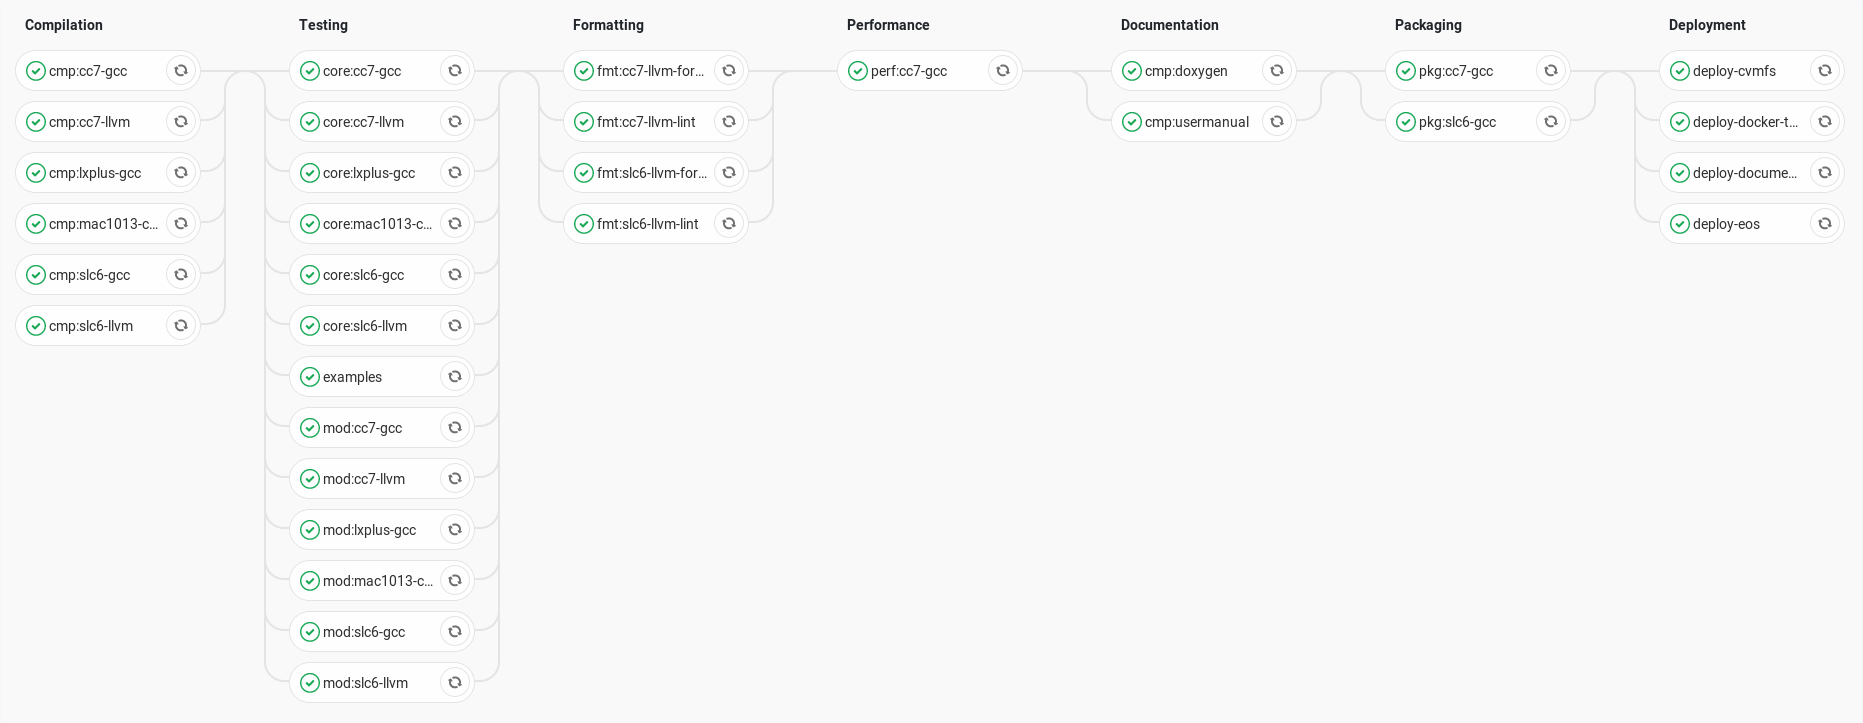
\includegraphics[width=\textwidth]{ci.png}
  \caption{Typical \apsq continous integration pipeline with 32 jobs distributed over seven distinct stages. In this example, all jobs passed.}
  \label{fig:ci}
\end{figure}

The \textbf{compilation} stage builds the framework from the source on different platforms.
Currently, builds are performed on Scientific Linux 6, CentOS7, and Mac OS X.
On Linux type platforms, the framework is compiled with recent versions of GCC and Clang, while the latest AppleClang is used on Mac OS X.
The build is always performed with the default compiler flags enabled for the project:
\begin{verbatim}
    -pedantic -Wall -Wextra -Wcast-align -Wcast-qual -Wconversion
    -Wuseless-cast -Wctor-dtor-privacy -Wzero-as-null-pointer-constant
    -Wdisabled-optimization -Wformat=2 -Winit-self -Wlogical-op
    -Wmissing-declarations -Wmissing-include-dirs -Wnoexcept
    -Wold-style-cast -Woverloaded-virtual -Wredundant-decls
    -Wsign-conversion -Wsign-promo -Wstrict-null-sentinel
    -Wstrict-overflow=5 -Wswitch-default -Wundef -Werror -Wshadow
    -Wformat-security -Wdeprecated -fdiagnostics-color=auto
    -Wheader-hygiene
\end{verbatim}

The \textbf{testing} stage executes the framework system and unit tests described in Section~\ref{sec:tests}.
Different jobs are used to run different test types.
This allows to optimize the CI setup depending on the demands of the test to be executed.
All tests are expected to pass, and no code that fails to satisfy all tests will be merged into the repository.

The \textbf{formatting} stage ensures proper formatting of the source code using the \command{clang-format} and following the coding conventions defined in the \file{.clang-format} file in the repository.
In addition, the \command{clang-tidy} tool is used for ``linting'' of the source code.
This means, the source code undergoes a static code analysis in order to identify possible sources of bugs by flagging suspicious and non-portable constructs used.
Tests are marked as failed if either of the CMake targets \command{make check-format} or \command{make check-lint} fail.
No code that fails to satisfy the coding conventions and formatting tests will be merged into the repository.

The \textbf{performance} stage runs a longer simulation with several thousand events and measures the execution time.
This facilitates monitoring of the simulation performance, a failing job would indicate a degradation in speed.
These CI jobs run on dedicated machines with only one concurrent job as described in Section~\ref{sec:tests}.
Performance tests are separated into their own CI stage because their execution is time consuming and they should only be started once proper  formatting of the new code is established.

The \textbf{documentation} stage prepares this user manual as well as the Doxygen source code documentation for publication.
This also allows to identify e.g.\ failing compilation of the \LaTeX documents or additional files which accidentally have not been committed to the repository.

The \textbf{packaging} stage wraps the compiled binaries up into distributable tarballs for several platforms.
This includes adding all libraries and executables to the tarball as well as preparing the \file{setup.sh} script to prepare run-time dependencies using the information provided to the build system.
This procedure is described in more detail in Section~\ref{sec:packaging}.

Finally, the \textbf{deployment} stage is only executed for new tags in the repository.
Whenever a tag is pushed, this stages receives the build artifacts of previous stages and publishes them to the \apsq project website through the EOS file system~\cite{eos}. More detailed information on deployments is provided in the following.

\section{Automatic Deployment}

The CI is configured to automatically deploy new versions of \apsq and its user manual and code reference to different places to make them available to users.
This section briefly describes the different deployment end-points currently configured and in use.
The individual targets are triggered either by automatic nightly builds or by publishing new tags.
In order to prevent accidental publications, the creation of tags is protected.
Only users with \emph{Maintainer} privileges can push new tags to the repository.
For new tagged versions, all deployment targets are executed.

\subsection{Software deployment to CVMFS}
\label{sec:cvmfs}

The software is automatically deployed to CERN's VM file system (CVMFS)~\cite{cvmfs} for every new tag.
In addition, the \parameter{master} branch is built and deployed every night.
New versions are published to the folder \dir{/cvmfs/clicdp.cern.ch/software/allpix-squared/} where a new folder is created for every new tag, while updates via the \parameter{master} branch are always stored in the \dir{latest} folder.

The deployed version currently comprises all modules as well as the detector models shipped with the framework.
An additional \file{setup.sh} is placed in the root folder of the respective release, which allows to set up all runtime dependencies necessary for executing this version.
Versions both for SLC\,6 and CentOS\,7 are provided.

The deployment CI job runs on a dedicated computer with a GitLab SSH runner.
Job artifacts from the packaging stage of the CI are downloaded via their ID using the script found in \dir{.gitlab/ci/download_artifacts.py}, and are made available to the \emph{cvclicdp} user which has access to the CVMFS interface.
The job checks for concurrent deployments to CVMFS and then unpacks the tarball releases and publishes them to the CLICdp experiment CVMFS space, the corresponding script for the deployment can be found in \dir{.gitlab/ci/gitlab_deployment.sh}.
This job requires a private API token to be set as secret project variable through the GitLab interface, currently this token belongs to the service account user \emph{ap2}.

\subsection{Documentation deployment to EOS}

The project documentation is deployed to the project's EOS space at \dir{/eos/project/a/allpix-squared/www/} for publication on the project website.
This comprises both the PDF and HTML versions of the user manual (subdirectory \dir{usermanual}) as well as the Doxygen code reference (subdirectory \dir{reference/}).
The documentation is only published only for new tagged versions of the framework.

The CI jobs uses the \parameter{ci-web-deployer} Docker image from the CERN GitLab CI tools to access EOS, which requires a specific file structure of the artifact.
All files in the artifact's \dir{public/} folder will be published to the \dir{www/} folder of the given project.
This job requires the secret project variables \parameter{EOS_ACCOUNT_USERNAME} and \parameter{EOS_ACCOUNT_PASSWORD} to be set via the GitLab web interface.
Currently, this uses the credentials of the service account user \emph{ap2}.

\subsection{Release tarball deployment to EOS}

Binary release tarballs are deployed to EOS to serve as downloads from the website to the directory \dir{/eos/project/a/allpix-squared/www/releases}.
New tarballs are produced for every tag as well as for nightly builds of the \parameter{master} branch, which are deployed with the name \file{allpix-squared-latest-<system-tag>-opt.tar.gz}.

The files are taken from the packaging jobs and published via the \parameter{ci-web-deployer} Docker image from the CERN GitLab CI tools.
This job requires the secret project variables \parameter{EOS_ACCOUNT_USERNAME} and \parameter{EOS_ACCOUNT_PASSWORD} to be set via the GitLab web interface.
Currently, this uses the credentials of the service account user \emph{ap2}.

\section{Building Docker images}
\label{sec:build-docker}

New \apsq Docker images are automatically created and deployed by the CI for every new tag and as a nightly build from the \parameter{master} branch.
New versions are published to project Docker container registry~\cite{ap2-container-registry}.
Tagged versions can be found via their respective tag name, while updates via the nightly build are always stored with the \parameter{latest} tag attached.

The final Docker image is formed from three consecutive images with different layers of software added.
The `base` image contains all build dependencies such as compilers, CMake, and git.
It derives from a CentOS7 Docker image and can be build using the \file{etc/docker/Dockerfile.base} file via the following commands:

\begin{verbatim}
# Log into the CERN GitLab Docker registry:
$ docker login gitlab-registry.cern.ch
# Compile the new image version:
$ docker build --file etc/docker/Dockerfile.base            \
               --tag gitlab-registry.cern.ch/allpix-squared/\
                     allpix-squared/allpix-squared-base     \
               .
# Upload the image to the registry:
$ docker push gitlab-registry.cern.ch/allpix-squared/\
              allpix-squared/allpix-squared-base
\end{verbatim}

The two main dependencies of the framework are ROOT6 and Geant4, which are added to the base image via the \parameter{deps} Docker image created from the file \file{etc/docker/Dockerfile.deps} via:
\begin{verbatim}
$ docker build --file etc/docker/Dockerfile.deps            \
               --tag gitlab-registry.cern.ch/allpix-squared/\
               allpix-squared/allpix-squared-deps           \
              .
$ docker push gitlab-registry.cern.ch/allpix-squared/\
              allpix-squared/allpix-squared-deps
\end{verbatim}
These images are created manually and only updated when necessary, i.e.\ if major new version of the underlying dependencies are available.

\begin{warning}
  The dependencies Docker images should not be flattend with commands like

  \command{docker export <container id> | docker import - <tag name>}

  because it strips any \parameter{ENV} variables set or used during the build process. They are used to set up the ROOT6 and Geant4 environments. When flattening, their executables and data paths cannot be found in the final \apsq image.
\end{warning}

Finally, the latest revision of \apsq is built using the file \file{etc/docker/Dockerfile}.
This job is performed automatically by the continuous integration and the created containers are directly uploaded to the project's Docker registry.
\begin{verbatim}
$ docker build --file etc/docker/Dockerfile                                \
               --tag gitlab-registry.cern.ch/allpix-squared/allpix-squared \
              .
\end{verbatim}

A short summary of potential use cases for Docker images is provided in Section~\ref{sec:docker}.

\section{Tests}
\label{sec:tests}

The build system of the framework provides a set of automated tests which are executed by the CI to ensure proper functioning of the framework and its modules.
The tests can also be manually invoked from the build directory of \apsq with
\begin{verbatim}
$ ctest
\end{verbatim}

The different subcategories of tests described below can be executed or ignored using the \command{-E} (exclude) and \command{-R} (run) switches of the \command{ctest} program:
\begin{verbatim}
$ ctest -R test_performance
\end{verbatim}

The configuration of the tests can be found in the \dir{etc/unittests/test_*} directories of the repository and are automatically discovered by CMake.
CMake automatically searches for \apsq configuration files in the different directories and passes them to the \apsq executable~(cf.\ Section~\ref{sec:allpix_executable}).

Adding a new test is as simple as adding a new configuration file to one of the different subdirectories and specifying the pass or fail conditions based on the tags described in the following paragraph.

\paragraph{Pass and Fail Conditions}

The output of any test is compared to a search string in order to determine whether it passed or failed.
These expressions are simply placed in the configuration file of the corresponding tests, a tag at the beginning of the line indicates whether it should be used for passing or failing the test.
Each test can only contain one passing and one failing expression.
If different functionality and thus outputs need to be tested, a second test should be added to cover the corresponding expression.

Different tags are provided for Mac OS X since the C++ standard does not define the exact implementation of random number distributions such as \texttt{std::normal\_distribution}.
Thus, the distributions produce different results on different platforms even when used with the same random number as input.

\begin{description}
  \item[Passing a test] The expression marked with the tag \parameter{#PASS}/\parameter{#PASSOSX} has to be found in the output in order for the test to pass. If the expression is not found, the test fails.
  \item[Failing a test] If the expression tagged with \parameter{#FAIL}/\parameter{#FAILOSX} is found in the output, the test fails. If the expression is not found, the test passes.
  \item[Depending on another test] The tag \parameter{#DEPENDS} can be used to indicate dependencies between tests. For example, the module test 09 described below implements such a dependency as it uses the output of module test 08-1 to read data from a previously produced \apsq data file.
  \item[Defining a timeout] For performance tests the runtime of the application is monitored, and the test fails if it exceeds the number of seconds defined using the \parameter{#TIMEOUT} tag.
  \item[Adding additional CLI options] Additional module command line options can be specified for the \parameter{allpix} executable using the \parameter{#OPTION} tag, following the format found in Section~\ref{sec:allpix_executable}. Multiple options can be supplied by repeating the \parameter{#OPTION} tag in the configuration file, only one option per tag is allowed. In exactly the same way options for the detectors can be set as well using the \parameter{#DETOPION} tag.
\end{description}

\paragraph{Framework Functionality Tests}

The framework functionality tests aim at reproducing basic features such as correct parsing of configuration keys or resolution of module instantiations.
Currently implemented tests comprise:

\begin{description}
    \item[\file{test_01-1_globalconfig_detectors.conf}] tests the framework behavior in case of a non-existent detector setup description file.
    \item[\file{test_01-2_globalconfig_modelpaths.conf}] tests the correct parsing of additional model paths and the loading of the detector model.
    \item[\file{test_01-3_globalconfig_log_format.conf}] switches the logging format.
    \item[\file{test_01-4_globalconfig_log_level.conf}] sets a different logging verbosity level.
    \item[\file{test_01-5_globalconfig_log_file.conf}] configures the framework to write log messages into a file.
    \item[\file{test_01-6_globalconfig_missing_model.conf}] tests the behavior of the framework in case of a missing detector model file.
    \item[\file{test_01-7_globalconfig_random_seed.conf}] sets a defined random seed to start the simulation with.
    \item[\file{test_01-8_globalconfig_random_seed_core.conf}] sets a defined seed for the core component seed generator, e.g. used for misalignment.
    \item[\file{test_02-1_specialization_unique_name.conf}] tests the framework behavior for an invalid module configuration: attempt to specialize a unique module for one detector instance.
    \item[\file{test_02-2_specialization_unique_type.conf}] tests the framework behavior for an invalid module configuration: attempt to specialize a unique module for one detector type.
    \item[\file{test_03-1_geometry_g4_coordinate_system.conf}] ensures that the \apsq and Geant4 coordinate systems and transformations are identical.
    \item[\file{test_03-2_geometry_rotations.conf}] tests the correct interpretation of rotation angles in the detector setup file.
    \item[\file{test_03-3_geometry_misaligned.conf}] tests the correct calculation of misalignments from alignment precisions given in the detector setup file.
    \item[\file{test_03-4_geometry_overwrite.conf}] checks that detector model parameters are overwritten correctly as described in Section~\ref{sec:detector_models}.
    \item[\file{test_04-1_configuration_cli_change.conf}] tests whether single configuration values can be overwritten by options supplied via the command line.
    \item[\file{test_04-2_configuration_cli_nochange.conf}] tests whether command line options are correctly assigned to module instances and do not alter other values.
    \item[\file{test_05-1_overwrite_same_denied.conf}] tests whether two modules writing to the same file is disallowed if overwriting is denied.
    \item[\file{test_04-2_configuration_cli_nochange.conf}] tests whether two modules writing to the same file is allowed if the last one reenables overwriting locally.
\end{description}


\paragraph{Module Functionality Tests}

These tests ensure the proper functionality of each module covered and thus protect the framework against accidental changes affecting the physics simulation.
Using a fixed seed (using the \parameter{random_seed} configuration keyword) together with a specific version of Geant4~\cite{geant4} allows to reproduce the same simulation event.

One event is produced per test and the \parameter{DEBUG}-level logging output of the respective module is checked against pre-defined expectation output using regular expressions.
Once modules are altered, their respective expectation output has to be adapted after careful verification of the simulation result.

Currently implemented tests comprise:

\begin{description}
    \item[\file{test_01_geobuilder.conf}] takes the provided detector setup and builds the Geant4 geometry from the internal detector description. The monitored output comprises the calculated wrapper dimensions of the detector model.
    \item[\file{test_02-1_electricfield_linear.conf}] creates a linear electric field in the constructed detector by specifying the bias and depletion voltages. The monitored output comprises the calculated effective thickness of the depleted detector volume.
    \item[\file{test_02-2_electricfield_init.conf}] loads an INIT file containing a TCAD-simulated electric field (cf.\ Section~\ref{sec:module_electric_field}) and applies the field to the detector model. The monitored output comprises the number of field cells for each pixel as read and parsed from the input file.
    \item[\file{test_02-3_electricfield_linear_depth.conf}] creates a linear electric field in the constructed detector by specifying the applied bias voltage and a depletion depth. The monitored output comprises the calculated effective thickness of the depleted detector volume.
    \item[\file{test_02-4_magneticfield_constant.conf}] creates a constant magnetic field for the full volume and applies it to the geometryManager. The monitored output comprises the message for successful application of the magnetic field.
    \item[\file{test_03-1_deposition.conf}] executes the charge carrier deposition module. This will invoke Geant4 to deposit energy in the sensitive volume. The monitored output comprises the exact number of charge carriers deposited in the detector.
    \item[\file{test_03-2_deposition_mc.conf}] executes the charge carrier deposition module as the previous tests, but monitors the type, entry and exit point of the Monte Carlo particle associated to the deposited charge carriers.
    \item[\file{test_03-3_deposition_track.conf}] executes the charge carrier deposition module as the previous tests, but monitors the start and end point of one of the Monte Carlo tracks in the event.
    \item[\file{test_03-4_deposition_source_point.conf}] tests the point source in the charge carrier deposition module by monitoring the deposited charges.
    \item[\file{test_03-5_deposition_source_square.conf}] tests the square source in the charge carrier deposition module by monitoring the deposited charges.
    \item[\file{test_03-6_deposition_source_sphere.conf}] tests the sphere source in the charge carrier deposition module by monitoring the deposited charges.
    \item[\file{test_03-7_deposition_source_macro.conf}] tests the G4 macro source in the charge carrier deposition module using the macro file \file{source_macro_test.txt}, monitoring the deposited charges.
    \item[\file{test_03-8_deposition_point.conf}] tests the deposition of a point charge at a specified position, checks the position of the deposited charge carrier in global coordinates.
    \item[\file{test_03-9_deposition_scan.conf}] tests the scan of a pixel volume by depositing charges for a given number of events, check for the calculated voxel size.
    \item[\file{test_03-10_deposition_scan_cube.conf}] tests the calculation of the scanning points by monitoring the warning of the number of events is not a perfect cube.
    \item[\file{test_03-11_deposition_mip.conf}] tests the deposition of charges along a line by monitoring the calculated step size and number of charge carriers deposited per step.
    \item[\file{test_03-12_deposition_mip_position.conf}] tests the generation of the Monte Carlo particle when depositing charges along a line by monitoring the start and end positions of the particle.
    \item[\file{test_03-13_deposition_fano.conf}] tests the simulation of fluctuations in charge carrier generation by monitoring the total number of generated carrier pairs when altering the Fano factor.
    \item[\file{test_03-14_deposition_spot.conf}] tests the deposition of charge carriers around a fixed position with a Gaussian distribution.
    \item[\file{test_04-1_propagation_project.conf}] projects deposited charges to the implant side of the sensor. The monitored output comprises the total number of charge carriers propagated to the sensor implants.
    \item[\file{test_04-2_propagation_generic.conf}] uses the Runge-Kutta-Fehlberg integration of the equations of motion implemented in the drift-diffusion model to propagate the charge carriers to the implants. The monitored output comprises the total number of charges moved, the number of integration steps taken and the simulated propagation time.
    \item[\file{test_04-3_propagation_generic-magnetic.conf}] uses the Runge-Kutta-Fehlberg integration of the equations of motion implemented in the drift-diffusion model to propagate the charge carriers to the implants under the influence of a constant magnetic field. The monitored output comprises the total number of charges moved, the number of integration steps taken and the simulated propagation time.
    \item[\file{test_04-4_propagation_project_integration.conf}] projects deposited charges to the implant side of the sensor with a reduced integration time to ignore some charge carriers. The monitored output comprises the total number of charge carriers propagated to the sensor implants.
    \item[\file{test_05_transfer_simple.conf}] tests the transfer of charges from sensor implants to readout chip. The monitored output comprises the total number of charges transferred and the coordinates of the pixels the charges have been assigned to.
    \item[\file{test_06-1_digitization_charge.conf}] digitizes the transferred charges to simulate the front-end electronics. The monitored output of this test comprises the total charge for one pixel including noise contributions and the smeared threshold it is compared to.
    \item[\file{test_06-2_digitization_adc.conf}] digitizes the transferred charges and tests the conversion into ADC units. The monitored output comprises the converted charge value in units of ADC counts.
    \item[\file{test_06-3_digitization_gain.conf}] digitizes the transferred charges and tests the amplification process by monitoring the total charge after signal amplification and smearing.
    \item[\file{test_07_histogramming.conf}] tests the detector histogramming module and its clustering algorithm. The monitored output comprises the total number of clusters and their mean position.
    \item[\file{test_08-1_writer_root.conf}] ensures proper functionality of the ROOT file writer module. It monitors the total number of objects and branches written to the output ROOT trees.
    \item[\file{test_08-2_writer_rce.conf}] ensures proper functionality of the RCE file writer module. The correct conversion of the PixelHit position and value is monitored by the test's regular expressions.
    \item[\file{test_08-3_writer_lcio.conf}] ensures proper functionality of the LCIO file writer module. Similar to the above test, the correct conversion of PixelHits (coordinates and charge) is monitored.
    \item[\file{test_08-4_writer_corryvreckan.conf}] ensures proper functionality of the Corryvreckan file writer module. The monitored output comprises the coordinates of the pixel produced in the simulation.
    \item[\file{test_08-5_writer_corryvreckan_mc.conf}] ensures the correct storage of Monte Carlo truth particle information in the Corryvreckan file writer module by monitoring the local coordinates of the MC particle associated to the pixel hit.
    \item[\file{test_08-6_writer_text.conf}] ensures proper functionality of the ASCII text writer module by monitoring the total number of objects and messages written to the text file..
    \item[\file{test_08-7_writer_lcio_detector_assignment.conf}] exercises the assignment of detector IDs to \apsq detectors in the LCIO output file. A fixed ID and collection name is assigned to the simulated detector.
    \item[\file{test_08-8_writer_lcio_no_mc_truth.conf}] ensures that simulation results are properly converted to LCIO and stored even without the Monte Carlo truth information available.
    \item[\file{test_09-1_reader_root.conf}] tests the capability of the framework to read data back in and to dispatch messages for all objects found in the input tree. The monitored output comprises the total number of objects read from all branches.
    \item[\file{test_09-2_reader_root_seed.conf}] tests the capability of the framework to detect different random seeds for misalignment set in a data file to be read back in. The monitored output comprises the error message including the two different random seed values.
    \item[\file{test_09-3_reader_root_ignoreseed.conf}] tests if core random seeds are properly ignored by the ROOTObjectReader module if requested by the configuration. The monitored output comprises the warning message emitted if a difference in seed values is discovered.
\end{description}

\paragraph{Performance Tests}

Similar to the module test implementation described above, performance tests use configurations prepared such, that one particular module takes most of the load (dubbed the ``slowest instantiation'' by \apsq), and a few of thousand events are simulated starting from a fixed seed for the pseudo-random number generator.
The \parameter{#TIMEOUT} keyword in the configuration file will ask CTest to abort the test after the given running time.

In the project CI, performance tests are limited to native runners, i.e. they are not executed on docker hosts where the hypervisor decides on the number of parallel jobs.
Only one test is performed at a time.

Despite these countermeasures, fluctuations on the CI runners occur, arising from different loads of the executing machines.
Thus, all performance CI jobs are marked with the \parameter{allow_failure} keyword which allows GitLab to continue processing the pipeline but will mark the final pipeline result as ``passed with warnings'' indicating an issue in the pipeline.
These tests should be checked manually before merging the code under review.

Current performance tests comprise:

\begin{description}
    \item[\file{test_01_deposition.conf}] tests the performance of charge carrier deposition in the sensitive sensor volume using Geant4~\cite{geant4}. A stepping length of \SI{1.0}{\um} is chosen, and \num{10000} events are simulated. The addition of an electric field and the subsequent projection of the charges are necessary since \apsq would otherwise detect that there are no recipients for the deposited charge carriers and skip the deposition entirely.
    \item[\file{test_02-1_propagation_generic.conf}] tests the very critical performance of the drift-diffusion propagation of charge carriers, as this is the most computing-intense module of the framework. Charge carriers are deposited and a propagation with 10 charge carriers per step and a fine spatial and temporal resolution is performed. The simulation comprises \num{500} events.
    \item[\file{test_02-2_propagation_project.conf}] tests the projection of charge carriers onto the implants, taking into account the diffusion only. Since this module is less computing-intense, a total of \num{5000} events are simulated, and charge carriers are propagated one-by-one.
    \item[\file{test_02-3_propagation_generic_multithread.conf}] tests the performance of multi-threaded simulation. It utilizes the very same configuration as performance test 02-1 but in addition enables multi-threading with four worker threads.
\end{description}
